% Straight up stealing preamble from Eli Holmes 
%%%%%%%%%%%%%%%%%%%%%%%%%%%%%%%%%%%%%%START PREAMBLE THAT IS THE SAME FOR ALL EXAMPLES
\documentclass{article}

%Required: You must have these
\usepackage{Sweave}
\usepackage{graphicx}
\usepackage{tabularx}
\usepackage{hyperref}
\usepackage{natbib}
\usepackage{pdflscape}
\usepackage{array}
\usepackage{gensymb}
\usepackage{amsmath}
%\usepackage[backend=bibtex]{biblatex}
%Strongly recommended
  %put your figures in one place
%\SweaveOpts{prefix.string=figures/, eps=FALSE} 
%you'll want these for pretty captioning
\usepackage[small]{caption}

\setkeys{Gin}{width=0.8\textwidth}  %make the figs 50 perc textwidth
\setlength{\captionmargin}{30pt}
\setlength{\abovecaptionskip}{10pt}
\setlength{\belowcaptionskip}{10pt}
% manual for caption  http://www.dd.chalmers.se/latex/Docs/PDF/caption.pdf

%Optional: I like to muck with my margins and spacing in ways that LaTeX frowns on
%Here's how to do that
 \topmargin -1.5cm        
 \oddsidemargin -0.04cm   
 \evensidemargin -0.04cm  % same as oddsidemargin but for left-hand pages
 \textwidth 16.59cm
 \textheight 21.94cm 
 %\pagestyle{empty}       % Uncomment if don't want page numbers
 \parskip 7.2pt           % sets spacing between paragraphs
 %\renewcommand{\baselinestretch}{1.5} 	% Uncomment for 1.5 spacing between lines
\parindent 0pt% sets leading space for paragraphs
\usepackage{setspace}
%\doublespacing

%Optional: I like fancy headers
%\usepackage{fancyhdr}
%\pagestyle{fancy}
%\fancyhead[LO]{How do climate change experiments actually change climate}
%\fancyhead[RO]{2016}
 
%%%%%%%%%%%%%%%%%%%%%%%%%%%%%%%%%%%%%%END PREAMBLE THAT IS THE SAME FOR ALL EXAMPLES

%Start of the document
\begin{document}

%\SweaveOpts{concordance=TRUE}
\bibliographystyle{..//..//refs/bibstyles/amnat.bst}% i moved a style file into the ospree git repo. feel free to add whatever style you like and update, lizzie! I don't have besjournals

\title{Supplemental materials  for Chilling outweighs photoperiod and forcing cues for temperate trees in experiments, but not in natural systems} % perspective paper for OSPREE analyses
% or Chilling dominates tree budburst in controlled climate experiments, but not in the great outdoors

\author{A.K. Ettinger, C. Chamberlain, I. Morales-Castilla, D. Buonaiuto, D. Flynn, T. Savas, \\J. Samaha \& E. Wolkovich}
%\date{\today} 
\maketitle  %put the fancy title on
%\tableofcontents      %add a table of contents
%\clearpage
%%%%%%%%%%%%%%%%%%%%%%%%%%%%%%%%%%%%%%%%%%%%%%%%%%%
\renewcommand{\thetable}{S\arabic{table}}
\renewcommand{\thefigure}{S\arabic{figure}}

\section*{Supplemental Methods}
% Include:
% Why we studied budburst and what it means ... Cat put together a 'what is budburst' file we should include with database. (Full OSPREE: 13,000 rows across 85 studies across 41 years and 227 species) - % CJC - I can look this over and make it more readable!

\subsection*{The OSPREE Database}

\par Some species are only represented in one dataset in the OSPREE database, making it impossible to differentiate between species and treatment statistical effects for these taxa. To address this, we combined species found in only one study into ``complexes" at the level of genera. Thus our taxonomic units of analysis are ``species complexes"; either species represented in >1 dataset or generic complexes combing multiple species that are each singly represented in the dataset. Species represented in only one dataset with no congenerics in other datasets were excluded from our analysis.


\subsection*{Models}

\par The models were fit using the programming languages \texttt{Stan} \citep{Carpenter:2016aa}(\texttt{www.mc-stan.org}), accessed via the \textit{rstan} package (version 2.17.3) in R \citep{Rcore:2017,rstan2018}, version XXXX. Stan provides efficient MCMC sampling via a No-U-Turn Hamiltonian Monte Carlo approach (more details can be found in \citet{BDA} and in \citet{Carpenter:2016aa}). We validated that our model code using test data, then fit the following models:
\begin{enumerate}
\item \underline{Main budburst model}:
\begin{align*}
y_i &= N(\alpha_{sp[i]} + \beta_{forcing_{sp[i]}} + \beta_{photoperiod_{sp[i]}} + \beta_{chilling_{sp[i]} + \epsilon_i}, \epsilon_i \sim N(0,\sigma^2_y)
\end{align*}


\noindent The $\alpha$ and each of the three $\beta$ coefficients were modeled at the species level, as follows:
\begin{align*}
\alpha_{sp} \sim N(\mu_{\alpha}, \sigma_{\alpha}) \\
\beta_{forcing_{sp}} \sim N(\mu_{forcing}, \sigma_{forcing}) \\
\beta_{photoperiod_{sp}} \sim N(\mu_{photoperiod}, \sigma_{photoperiod})\\
\beta_{chilling{sp}} \sim N(\mu_{chilling}, \sigma_{chilling})
\end{align*}

\item \underline{Latitude model}:

\item \underline{Weinberger  model}:

\end{enumerate}

\noindent For all models, we choose weakly informative priors; increasing the priors three-fold did not change the model results. 

We ran four chains simultaneously, each with 1 500 warm-up iterations followed by 2 500 sampling iterations, yeilding 4 000 posterior samples for each parameter. We assessed model performance through $\hat{R}$ close to 1 and high $n_{eff}$ (4 000 for most parameters, but as low as 1 057 for several parameters) as well as visual consideration of chain convergence and posteriors \citep{BDA}. 

In our figures  we show means $\pm$ XX\% credible intervals from our models, because of our focus here is on the most likely value for each parameter (e.g., estimated response to forcing) and because they are computationally stable \citep{BDA,Carpenter:2016aa}. See tables XX other XX\% credible intervals. 


\par Quick review of what standardized units are (We used a standardized scale to allow comparisons of the three cues ...)

\subsection*{Forecasting with the OSPREE model}
We selected sites in Europe where temperature and budburst have been monitored since the 1950s (the Pan European Phenology Project, http://www.pep725.eu, PEP). We extracted mean temperature data from 1951 through 1961 (pre-warming time period) and used these values as baseline data. We then investigated model predictions of budburst given different levels of warming (from 1-7 \degree C) above this baseline, including altered chilling and forcing as well as potential declines in photoperiod due to advancing phenology. We did this for one common European species: \emph{Betula pendula} (silver birch) at all latitudes and longitudes included in the PEP database between 1951 and 1961. We also did this for another common European species, \emph{Fagus sylvatica}, for a subset of sites where it occured with \emph{B. pendula}, in order to compare budburst responses of these two species when they experience the same baseline climate and warming levels.

\par To understand how experimental temperature, photoperiod, and budburst sensitivity compare to past and current conditions in nature, we used data from the PEP database. We summarized forcing, chilling, and budburst doy for two common species: \emph{Betula pendula} (silver birch) and \emph{Fagus sylvatica} (European beech) during a pre-warming time-period (1950-1980) and post-warming period (1981-2014?). 

\section*{Supplemental Results/Discussion}
\begin{enumerate}
\item Surprising species-specific responses: 
\begin{enumerate}

\item Positive responses to forcing: Fagus, Acer-complex, Fraxinus complex, Cornus alba.
\item Positive Responses to chilling for Tilia and Salix.  have positive response to chilling with chill portions model.

\end{enumerate}
\end{enumerate}

\section*{Understanding declines in temperature sensitivity in European long-term data}
% See files: PEP_climate/comparetopepsims.R and pep_sims/pepvarsim.R 
% HELP from Cat needed !!! I guessed at the methods for PEP sites ... She should double-check everything I wrote
As our model results (when applied to realistic forcing, chilling and photoperiod conditions in Europe) do not predict a dramatic decline temperature sensitivity, we tested whether observed declines could instead be due to a statistical artifact of the method commonly used to estimate temperature sensitivity (a linear regression of annual budburst date versus mean or other aggregated metrics of spring temperature yielding estimates in days/$^{\circ}$C). If warming produces systematically warmer daily temperatures this method will inherently estimate lower sensitivities, because the `days' unit will effectively have increased in the thermal time it represents.

\par To test this hypothesis we compared observed trends with simulations. First, we collated PEP 725 (CITE) data for \emph{Betula pendula} for all sites with leafout data each year from two 10-year time-periods: 1951-1960, which represented a period before significant anthropogenic warming (citeIPCC) and 2001-2010, a period with significant warming. We used leafout data (BBCH=11; which is defined as ``leaf unfolding (first visible leaf stalk" in the PEP725 database)) instead of budburst (BBCH=7; defined as ``Beginning of sprouting") as leafout data are far more common in the PEP 725 database. %CJC - this is great! exactly what I did, I just added defintions for the BBCHs we used
Next, we simulated budburst data with constant cues. For this, we did not include any chilling or photoperiod cues, but simply assumed budburst occurred after a certain summation of heat, estimated via growing degree days with a base temperature of 0$^{\circ}$C. We then estimated temperature sensitivity (days/$^{\circ}$C)) and the difference in these estimates given different levels of spring warming. For the simulations showed here we used a GDD requirement of 150, a base mean spring temperature of 6$^{\circ}$C with a variance of 3$^{\circ}$C and estimated temperature sensitivity for 10-year periods for 45 simulated sites (these values were chosen to best match the PEP 725 data, but note that the general findings are robust to other combinations of these parameter values).

\par As expected temperature sensitivity estimates for \emph{Betula pendula} from PEP 725 declined across the two time periods in step with warming daily temperatures. Across the sites studied here we estimated a decline of 0.9$\pm$0.3 days/$^{\circ}$C (comparing 2000-2010 and 1950-1960) and 1.1$^{\circ}$C warming; this estimate was very similar to simulations given constant cues and 1$^{\circ}$C warming (Fig. \ref{fig:pepsims}). Additionally, in both the real and simulated data variance in leafout date declined, as would be expected if plants use a thermal sum threshold of forcing to leaf out and warming produces systematically warmer days: in the PEP 725 data we found a decline in leafout variance of 57\%, compared to a decline of 37\% in the simulations. Additionally we found little change in accumulated chilling (1 September - 1 March of each year) in the PEP 725 data across the two time points (2247$\pm$31 Utah units in 1950-1960, compared to 2236$\pm$20 Utah units in 2000-2010), further suggesting that shifts in chilling do not explain the declining sensitivities. Simple plots of the chilling and forcing required for budburst suggest very low chilling is often required to dramatically increase the forcing required for budburst (Fig. {fig:pepgddchill}).
% Need to add SE or such to % ... See PEP_climate/comparetopepsims.R


\section*{May need to move back to main text ...}

\par The paucity of studies directly manipulating chilling---which our results suggest has the greatest effect on budburst---suggests a major gap in current research. While many studies (X out of Y here) directly manipulated forcing, far fewer directly manipulated chilling (Z out of Y). 
% [Next bit is in main text currently.] Instead many studies (J out of Y) estimate chilling effects through sequential removal of tissue from the field and exposure to `forcing' conditions (cite Weinberger), with the assumption that tissue collected later experienced more chilling. The challenge with this method is that photoperiod and other factors have also changed during this time. Indeed, we found estimates varied in XX way when derived from direct manipulations of chilling versus the sequential `Weinberger' method. 
Our model highlights how the choice of chill units can affect model estimates and associated forecasts (reference supplemental figure with utah units vs chill portions in main manuscript). 
Given the limited manipulation of chilling in studies, we estimated chilling for all studies by combining chilling from the field (i.e., chilling before plants were sampled) and experimental chilling into two widely used metrics of chilling: Utah and Chill portions \citep{dennis2003}. We found the effects of chilling and other cues remain qualitatively consistent across the two chilling units, though chilling and photoperiod estimates were slightly lower using chill portions compared to Utah (cite supplemental table comparing estimates with both units).  

%Most studies do not experimentally apply chilling by manipulating duration or temperature of chilling, nor do most estimate the chilling imposed in their experiment. We therefore calculated the chilling imposed by most studies, as it would otherwise have been impossible to provide estimates with only experimental chilling (reference lizzie's supp heat maps). %this last part may be better for methods?


% I think the below belongs where we discuss the PEP results. I think we discussed most of the points below already in one form or another above?
%\par We expect climate change to continue to have dramatic effects on spring phenology, because the two temperature-derived cues (chilling and forcing) both strongly affect budburst \citep{Laube:2014a}. However, the relative importance of chilling versus forcing (i.e., the extent to which a chilling threshold will be reached and cause delays in budburst with additional warming) will vary spatially. Forcing is increasing with climate change and is therefore expected to continue advancing budburst. Chilling, on the other hand, is expected to increase in some locations and decrease in others with climate change \citep{fraga2019}, so budburst responses may advance less strongly in places where chilling declines. In some locations, budburst may even delay with substantial amounts of warming (e.g. X degrees, as is forecasted for the end of the 21st century, IPCC, Fig. \ref{fig:fore}) as chilling limitations come into play. 

\par An additional important limitation is the rarity of studies designed to test interactions. Interactions between these cues are widely expected (cites) and, when examined, often found (cites), we were unable to estimate interactions in our meta-analysis because very few studies design experiments to test for interactions between chilling, forcing, and photoperiod (cite table with number of interactions from coding challenge!). The few that do incorporate interactions generally use the Weinberger method, which is not designed to robustly tease out of the effects of multiple cues (cites, Tables, figs).  Our estimated effects average over interactions \citep{gelman2006}, but identifying them in future research will be critical to understanding and predicting budburst. For example, the most commonly observed interaction between chilling and forcing---that lower amounts of chilling increases forcing requirements for budburst %\citep{} 
(cite papers in the ospree database that interact chilling and forcing)
---is the hypothesized cause of declining sensitivities in European trees \citep{fu2015,vitasse}. As more data become available, it would allow additional tests of important interactions, such as how responses vary across latitudes (ref latitude figure). % Maybe add: In addition to data limitation, disentangling forcing from chilling conditions is a challenge because information on endodormancy requirements is very scarce \citep{chuine2016}.% Though I wonder if this belongs above in discussion of chilling?

\section*{Things we'd like to discuss in main paper but don't have room for}

% I suggest we save a discussion of Photothermoperiodicity for a plant-specific journal in which we have a much larger number of words ... %CJC - I'm glad this made it in the supplement but I don't think it needs to be in the main text with the way it's written now! I agree it'd be cool to add it to the main text if we go with another journal
\par \underline{Photothermoperiodicity}, for example, is an ongoing challenge: chamber studies may seek to replicate patterns in nature, pairing daylength and temperature treatments such that night temperatures are always cooler than day temperatures (e.g., cite studies that do this).  This results in daylength treatments that differ in temperature conditions (and therefore chilling and forcing treatments) as well, however.  

\par \underline{Chilling:} Current common models for chilling (i.e., Utah which was developed for XX species,  chill portions which was developed for XX species) are \emph{hypotheses} for how chilling may accumulate to affect the process of dormancy release, but are likely to be inaccurate for many species. Our model highlights how the choice of chill units can affect model estimates and associated forecasts (Figures 1,\ref{fig:figmucpz}\ref{fig:muutnonz}, \ref{fig:mucpnonz}). 


\bibliography{..//..//refs/ospreebibplus.bib}

\newpage
\section* {Supplemental Tables}
\begin{footnotesize} 
% latex table generated in R 3.4.2 by xtable 1.8-2 package
% Fri Jun 21 09:17:00 2019
\begin{table}[ht]
\centering
\caption{\textbf{Species included in the OSPREE database}. Could add to this: the range of forcing, chilling, and photoperiod treatments for each species, and perhaps the range of latitudes, in OSPREE.
} 
\label{tab:sp}
\begingroup\footnotesize
\begin{tabular}{|p{0.20\textwidth}|p{0.08\textwidth}|p{0.3\textwidth}|}
  \hline
spname & stnum & studies \\ 
  \hline
Abies.alba &   2 & basler12,laube14a \\ 
  Abies.homolepis &   1 & laube14a \\ 
  Acer.barbinerve &   1 & zohner16 \\ 
  Acer.campestre &   1 & zohner16 \\ 
  Acer.ginnala &   1 & zohner16 \\ 
  Acer.negundo &   1 & laube14a \\ 
  Acer.platanoides &   1 & zohner16 \\ 
  Acer.pseudoplatanus &   3 & basler12,basler14,laube14a \\ 
  Acer.saccharinum &   1 & webb78 \\ 
  Acer.saccharum &   3 & calme94,laube14a,webb78 \\ 
  Acer.tataricum &   1 & laube14a \\ 
  Actinidia.deliciosa &   2 & biasi12,guerriero90 \\ 
  Aesculus.flava &   1 & zohner16 \\ 
  Aesculus.hippocastanum &   3 & basler12,laube14a,zohner16 \\ 
  Aesculus.parviflora &   1 & zohner16 \\ 
  Alnus.glutinosa &   2 & heide93,myking98 \\ 
  Alnus.incana &   2 & heide93,zohner16 \\ 
  Alnus.maximowiczii &   1 & zohner16 \\ 
  Amelanchier.alnifolia &   1 & zohner16 \\ 
  Amelanchier.florida &   1 & zohner16 \\ 
  Amelanchier.laevis &   1 & zohner16 \\ 
  Amorpha.fruticosa &   1 & laube14a \\ 
  Aronia.melanocarpa &   1 & zohner16 \\ 
  Berberis.dielsiana &   1 & zohner16 \\ 
  Betula.alleghaniensis &   1 & calme94 \\ 
  Betula.lenta &   1 & zohner16 \\ 
  Betula.nana &   1 & zohner16 \\ 
  Betula.pendula &  10 & heide93,li05,rinne97,basler12,laube14a,laube14b,linkosalo06,myking95,myking95,skuterud94 \\ 
  Betula.populifolia &   1 & zohner16 \\ 
  Betula.pubescens &   6 & heide93,rinne94,caffarra11a,caffarra11b,myking95,myking97 \\ 
  Buddleja.albiflora &   1 & zohner16 \\ 
  Buddleja.alternifolia &   1 & zohner16 \\ 
  Buddleja.davidii &   1 & zohner16 \\ 
  Caragana.pygmaea &   1 & zohner16 \\ 
  Carpinus.betulus &   3 & heide93a,laube14a,zohner16 \\ 
  Carpinus.laxiflora &   1 & zohner16 \\ 
  Carpinus.monbeigiana &   1 & zohner16 \\ 
  Carya.cordiformis &   1 & zohner16 \\ 
  Carya.laciniosa &   1 & zohner16 \\ 
  Carya.ovata &   1 & zohner16 \\ 
  Castanea.sativa &   1 & zohner16 \\ 
  Cedrus.libani &   1 & zohner16 \\ 
  Celtis.caucasica &   1 & zohner16 \\ 
  Celtis.laevigata &   1 & zohner16 \\ 
  Celtis.occidentalis &   1 & zohner16 \\ 
  Cephalanthus.occidentalis &   1 & zohner16 \\ 
  Cercidiphyllum.japonicum &   1 & zohner16 \\ 
  Cercidiphyllum.magnificum &   1 & zohner16 \\ 
  Cercis.canadensis &   1 & zohner16 \\ 
  Cercis.chinensis &   1 & zohner16 \\ 
  Cladrastis.lutea &   1 & zohner16 \\ 
  Cornus.alba &   2 & laube14a,zohner16 \\ 
  Cornus.kousa &   1 & zohner16 \\ 
  Cornus.mas &   2 & laube14a,laube14b \\ 
  Corylopsis.sinensis &   1 & zohner16 \\ 
  Corylopsis.spicata &   1 & zohner16 \\ 
  Corylus.avellana &   4 & basler12,heide93,laube14a,zohner16 \\ 
  Corylus.heterophylla &   1 & zohner16 \\ 
  Corylus.sieboldiana &   1 & zohner16 \\ 
  Decaisnea.fargesii &   1 & zohner16 \\ 
  Deutzia.gracilis &   1 & zohner16 \\ 
  Deutzia.scabra &   1 & zohner16 \\ 
  Elaeagnus.ebbingei &   1 & zohner16 \\ 
  Eleutherococcus.senticosus &   1 & zohner16 \\ 
  Eleutherococcus.setchuenensis &   1 & zohner16 \\ 
  Eleutherococcus.sieboldianus &   1 & zohner16 \\ 
  Euonymus.europaeus &   1 & zohner16 \\ 
  Euonymus.latifolius &   1 & zohner16 \\ 
  Fagus.crenata &   1 & zohner16 \\ 
  Fagus.engleriana &   1 & zohner16 \\ 
  Fagus.orientalis &   1 & zohner16 \\ 
  Fagus.sylvatica &  10 & falusi03,falusi90,falusi96,falusi97,basler12,basler14,caffarra11a,heide93a,heide93a,zohner16 \\ 
  Forsythia.ovata &   1 & zohner16 \\ 
  Forsythia.suspensa &   1 & zohner16 \\ 
  Fraxinus.americana &   1 & webb78 \\ 
  Fraxinus.chinensis &   1 & laube14a \\ 
  Fraxinus.excelsior &   2 & basler12,laube14a \\ 
  Fraxinus.latifolia &   1 & zohner16 \\ 
  Fraxinus.ornus &   1 & zohner16 \\ 
  Fraxinus.pennsylvanica &   1 & laube14a \\ 
  Ginkgo.biloba &   1 & zohner16 \\ 
  Hamamelis.japonica &   1 & zohner16 \\ 
  Hamamelis.vernalis &   1 & zohner16 \\ 
  Heptacodium.miconioides &   1 & zohner16 \\ 
  Hibiscus.syriacus &   1 & zohner16 \\ 
  Hydrangea.arborescens &   1 & zohner16 \\ 
  Hydrangea.involucrata &   1 & zohner16 \\ 
  Hydrangea.serrata &   1 & zohner16 \\ 
  Juglans.ailantifolia &   1 & laube14a \\ 
  Juglans.cinerea &   1 & laube14a \\ 
  Juglans.regia &   1 & laube14a \\ 
  Larix.decidua &   4 & basler12,gomory15,laube14a,laube14b \\ 
  Larix.gmelinii &   1 & zohner16 \\ 
  Larix.kaempferi &   1 & zohner16 \\ 
  Ligustrum.tschonoskii &   1 & zohner16 \\ 
  Liquidambar.orientalis &   1 & zohner16 \\ 
  Liquidambar.styraciflua &   1 & zohner16 \\ 
  Liriodendron.tulipifera &   1 & zohner16 \\ 
  Lonicera.alpigena &   1 & zohner16 \\ 
  Lonicera.caerulea &   1 & zohner16 \\ 
  Lonicera.maximowiczii &   1 & zohner16 \\ 
  Malus.domestica &   3 & cook00b,gianfagna85,swartz81 \\ 
  Metasequoia.glyptostroboides &   1 & zohner16 \\ 
  Nothofagus.antarctica &   1 & zohner16 \\ 
  Oemleria.cerasiformis &   1 & zohner16 \\ 
  Olea.europaea &   1 & ramos99 \\ 
  Orixa.japonica &   1 & zohner16 \\ 
  Ostrya.carpinifolia &   1 & zohner16 \\ 
  Ostrya.virginiana &   1 & zohner16 \\ 
  Paeonia.rockii &   1 & zohner16 \\ 
  Parrotia.persica &   1 & zohner16 \\ 
  Parrotiopsis.jaquemontiana &   1 & zohner16 \\ 
  Photinia.villosa &   1 & zohner16 \\ 
  Picea.abies &   9 & basler12,basler14,gomory15,laube14a,laube14b,partanen01,partanen98,worrall67,worrall67, \\ 
  Picea.glauca &   1 & man10 \\ 
  Pinus.nigra &   1 & laube14a \\ 
  Pinus.strobus &   1 & laube14a \\ 
  Pinus.sylvestris &   1 & laube14a \\ 
  Pinus.wallichiana &   1 & laube14a \\ 
  Populus.deltoides &   1 & thielges75 \\ 
  Populus.koreana &   1 & zohner16 \\ 
  Populus.tremula &   3 & heide93,laube14a,laube14b \\ 
  Prinsepia.sinensis &   1 & zohner16 \\ 
  Prinsepia.uniflora &   1 & zohner16 \\ 
  Prunus.avium &   2 & basler12,laube14a \\ 
  Prunus.cerasifera &   1 & zohner16 \\ 
  Prunus.padus &   3 & heide93,myking98,zohner16 \\ 
  Prunus.persica &   1 & chavarria09 \\ 
  Prunus.serotina &   1 & laube14a \\ 
  Prunus.serrulata &   1 & zohner16 \\ 
  Prunus.tenella &   1 & zohner16 \\ 
  Pseudotsuga.menziesii &   3 & guak98,campbell75,laube14a \\ 
  Ptelea.trifoliata &   1 & zohner16 \\ 
  Pyrus.elaeagnifolia &   1 & zohner16 \\ 
  Pyrus.pyrifolia &   1 & zohner16 \\ 
  Pyrus.ussuriensis &   1 & zohner16 \\ 
  Quercus.bicolor &   1 & laube14a \\ 
  Quercus.coccifera &   1 & sanzperez10 \\ 
  Quercus.faginea &   2 & Sanz-Perez09,sanzperez10 \\ 
  Quercus.ilex &   3 & Sanz-Perez09,sanzperez10,morin10 \\ 
  Quercus.petraea &   2 & basler12,basler14 \\ 
  Quercus.pubescens &   1 & morin10 \\ 
  Quercus.robur &   4 & laube14a,laube14b,morin10,zohner16 \\ 
  Quercus.rubra &   2 & calme94,laube14a \\ 
  Quercus.shumardii &   1 & zohner16 \\ 
  Rhamnus.alpina &   1 & zohner16 \\ 
  Rhamnus.cathartica &   1 & zohner16 \\ 
  Rhododendron.canadense &   1 & zohner16 \\ 
  Rhododendron.dauricum &   1 & zohner16 \\ 
  Rhododendron.mucronulatum &   1 & zohner16 \\ 
  Ribes.alpinum &   1 & zohner16 \\ 
  Ribes.divaricatum &   1 & zohner16 \\ 
  Ribes.glaciale &   1 & zohner16 \\ 
  Ribes.nigrum &   4 & jones12,heide12,pagter15,sonsteby14 \\ 
  Robinia.pseudoacacia &   2 & laube14a,laube14b \\ 
  Rosa.hugonis &   1 & zohner16 \\ 
  Rosa.majalis &   1 & zohner16 \\ 
  Rubus.idaeus &   1 & heide93 \\ 
  Salix.gracilistyla &   1 & zohner16 \\ 
  Salix.repens &   1 & zohner16 \\ 
  Salix.smithiana &   1 & caffarra11a \\ 
  Sambucus.nigra &   1 & zohner16 \\ 
  Sambucus.pubens &   1 & zohner16 \\ 
  Sambucus.tigranii &   1 & zohner16 \\ 
  Sinowilsonia.henryi &   1 & zohner16 \\ 
  Sorbus.aria &   1 & zohner16 \\ 
  Sorbus.aucuparia &   2 & basler12,heide93 \\ 
  Sorbus.commixta &   1 & zohner16 \\ 
  Sorbus.decora &   1 & zohner16 \\ 
  Spiraea.canescens &   1 & zohner16 \\ 
  Spiraea.chamaedryfolia &   1 & zohner16 \\ 
  Spiraea.japonica &   1 & zohner16 \\ 
  Stachyurus.praecox &   1 & zohner16 \\ 
  Stachyurus.sinensis &   1 & zohner16 \\ 
  Symphoricarpos.albus &   2 & laube14a,laube14b \\ 
  Syringa.josikaea &   1 & zohner16 \\ 
  Syringa.reticulata &   1 & zohner16 \\ 
  Syringa.villosa &   1 & zohner16 \\ 
  Syringa.vulgaris &   3 & basler12,laube14a,laube14b \\ 
  Tilia.cordata &   2 & basler12,caffarra11a \\ 
  Tilia.dasystyla &   1 & zohner16 \\ 
  Tilia.japonica &   1 & zohner16 \\ 
  Tilia.platyphyllos &   1 & zohner16 \\ 
  Toona.sinensis &   1 & zohner16 \\ 
  Ulmus.americana &   1 & zohner16 \\ 
  Ulmus.glabra &   1 & ghelardini10 \\ 
  Ulmus.laevis &   1 & zohner16 \\ 
  Ulmus.macrocarpa &   1 & ghelardini10 \\ 
  Ulmus.minor &   1 & ghelardini10 \\ 
  Ulmus.parvifolia &   1 & ghelardini10 \\ 
  Ulmus.pumila &   1 & ghelardini10 \\ 
  Ulmus.villosa &   1 & ghelardini10 \\ 
  Vaccinium.ashei &   1 & spiers74 \\ 
  Vaccinium.corymbosum &   1 & spann04 \\ 
  Viburnum.betulifolium &   1 & zohner16 \\ 
  Viburnum.buddleifolium &   1 & zohner16 \\ 
  Viburnum.carlesii &   1 & zohner16 \\ 
  Viburnum.opulus &   1 & zohner16 \\ 
  Viburnum.plicatum &   1 & zohner16 \\ 
  Vitis.vinifera &   2 & biasi12,schnabel87 \\ 
  Weigela.coraeensis &   1 & zohner16 \\ 
  Weigela.florida &   1 & zohner16 \\ 
  Weigela.maximowiczii &   1 & zohner16 \\ 
  \end{tabular}
\endgroup
\end{table}
\end{footnotesize} 


% latex table generated in R 3.4.2 by xtable 1.8-2 package
% Fri Jun 21 09:17:40 2019
\begin{table}[ht]
\centering
\caption{\textbf{Estimates from model fit with standardized predictors}. The model we present in the main text uses Utah units for chilling and includes studies that experimentally manipulated forcing and photoperiod. Using instead a model with chilling in Chill Portions (column two) results in quantitatively different species-level and overall estimates, though the results are qualitatively similar. We also present coefficients from a model including all species (i.e., with crops) with all treatment types. We present estimates and their 95 percent credible intervals from models in which the predictors have been standardized so that they are directly comparable,} 
\label{tab:methods}
\begingroup\footnotesize
\begin{tabular}{|p{0.15\textwidth}|p{0.08\textwidth}|p{0.1\textwidth}|p{0.08\textwidth}|p{0.1\textwidth}|p{0.08\textwidth}|p{0.1\textwidth}|}
  \hline
parameter & utah.est & utah.ci & cp.est & cp.ci & allsp.est & allsp.ci \\ 
  \hline
mu\_a\_sp & 29.92 & 26.41-33.37 & 30.74 & 26.91-34.4 & 30.86 & 28.61-33.17 \\ 
  mu\_b\_force\_sp & -4.37 & -6.7--2.12 & -4.8 & -7.1--2.44 & -6.15 & -8.56--3.72 \\ 
  mu\_b\_photo\_sp & -3.13 & -5.63--0.77 & -3.18 & -5.39--1.03 & -1.03 & -2.31-0.2 \\ 
  mu\_b\_chill\_sp & -8.87 & -12.06--5.77 & -8.2 & -11.25--4.97 & -8.04 & -9.65--6.42 \\ 
  sigma\_a\_sp & 9.41 & 7.21-12.2 & 10.17 & 7.69-13.29 & 14.42 & 12.67-16.42 \\ 
  sigma\_b\_force\_sp & 5.68 & 4.01-7.77 & 6.03 & 4.33-8.15 & 8.51 & 6.53-10.88 \\ 
  sigma\_b\_photo\_sp & 5.22 & 3.36-7.85 & 4.51 & 2.97-6.63 & 3.69 & 2.83-4.67 \\ 
  sigma\_b\_chill\_sp & 7.38 & 5.27-10.1 & 7.9 & 5.68-10.73 & 6.27 & 4.8-7.85 \\ 
  sigma\_y & 15.77 & 15.24-16.32 & 15.47 & 14.93-16 & 14.93 & 14.55-15.32 \\ 
   \hline
n\_sp & 39 &  & 39 &  & 205 &  \\ 
   \hline
\end{tabular}
\endgroup
\end{table}% latex table generated in R 3.4.2 by xtable 1.8-2 package
% Fri Jun 21 09:17:40 2019
\begin{table}[ht]
\centering
\caption{\textbf{Estimates from models fit with predictors on their natural scales},  so that effect sizes can be readily intepreted in a meaningful way (e.g., change in days of budburst per degree C of warming for forcing temperature). The model we present in the main text uses Utah units for chilling. Here we also present coeficients from a model included all species, including crops, and all treatment types. We present estimates and their 95 percent credible intervals from models in which the predictors have been standardized so that they are directly comparable,} 
\label{tab:methods}
\begingroup\footnotesize
\begin{tabular}{|p{0.15\textwidth}|p{0.08\textwidth}|p{0.1\textwidth}|p{0.08\textwidth}|p{0.1\textwidth}|p{0.08\textwidth}|p{0.1\textwidth}|}
  \hline
parameter & utah.est & utah.ci & cp.est & cp.ci & allsp.est & allsp.ci \\ 
  \hline
mu\_a\_sp & 62.89 & 54.9-70.93 & 67.02 & 58.05-75.76 & 62.57 & 57.64-67.38 \\ 
  mu\_b\_force\_sp & -0.79 & -1.16--0.42 & -0.85 & -1.25--0.45 & -1.02 & -1.29--0.76 \\ 
  mu\_b\_photo\_sp & -0.53 & -0.93--0.16 & -0.54 & -0.9--0.18 & -0.14 & -0.35-0.06 \\ 
  mu\_b\_chill\_sp & -2.86 & -3.78--1.95 & -0.25 & -0.33--0.16 & -2.49 & -2.92--2.06 \\ 
  sigma\_a\_sp & 19.17 & 14.76-25.04 & 21.93 & 16.9-28.18 & 17.7 & 15.31-20.42 \\ 
  sigma\_b\_force\_sp & 0.91 & 0.63-1.25 & 0.99 & 0.69-1.41 & 0.71 & 0.57-0.88 \\ 
  sigma\_b\_photo\_sp & 0.77 & 0.49-1.14 & 0.7 & 0.46-1.02 & 0.59 & 0.45-0.74 \\ 
  sigma\_b\_chill\_sp & 2.06 & 1.46-2.82 & 0.2 & 0.14-0.28 & 1.24 & 0.95-1.57 \\ 
  sigma\_y & 15.83 & 15.28-16.39 & 15.53 & 15.01-16.08 & 15.16 & 14.77-15.58 \\ 
   \hline
n\_sp & 39 &  & 39 &  & 205 &  \\ 
   \hline
\end{tabular}
\endgroup
\end{table}

Still need: Table 3S: a table that goes with Figure 3 (the 4-paneled 3D forecasting figure) that includes the mean budburst day of year, chilling estimates, mean winter temperature, and spring (forcing) temperatures for the 4 sites with no warming and with the 7 levels of warming.

% 
\newpage

\newpage
\section* {Supplemental Figures}

\newpage
\begin{figure}[h!]
\centering
\noindent 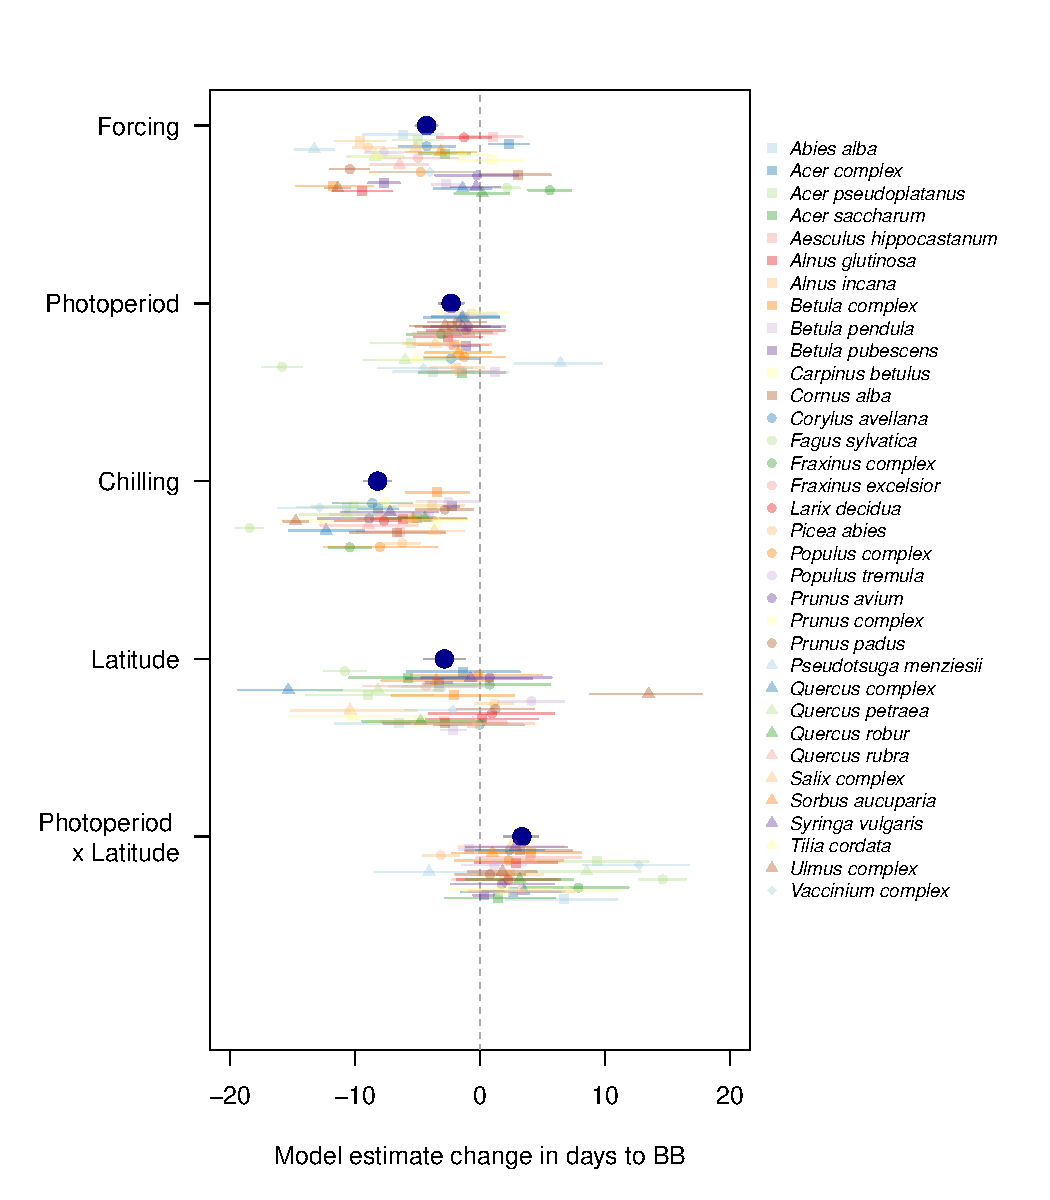
\includegraphics[width=0.75\textwidth]{..//..//analyses/lat_analysis/figures/latanalysis_spcom_expramp_fp.pdf}
\caption{\textbf{Estimates for effects of chilling exceeded estimates for forcing, photoperiod, latitude, and the interaction between latitude and photoperiod, for most species,} in the latitude budburst model fit to centered data, including the subset of studies in OSPREE database that XXX. Here we show estimates from the model fit to centered data, enabling comparisons of effects sizes across predictors, and using Utah units to quantify chilling.}
\label{fig:lat}
\end{figure}

\begin{figure}[h!]
\centering
\noindent 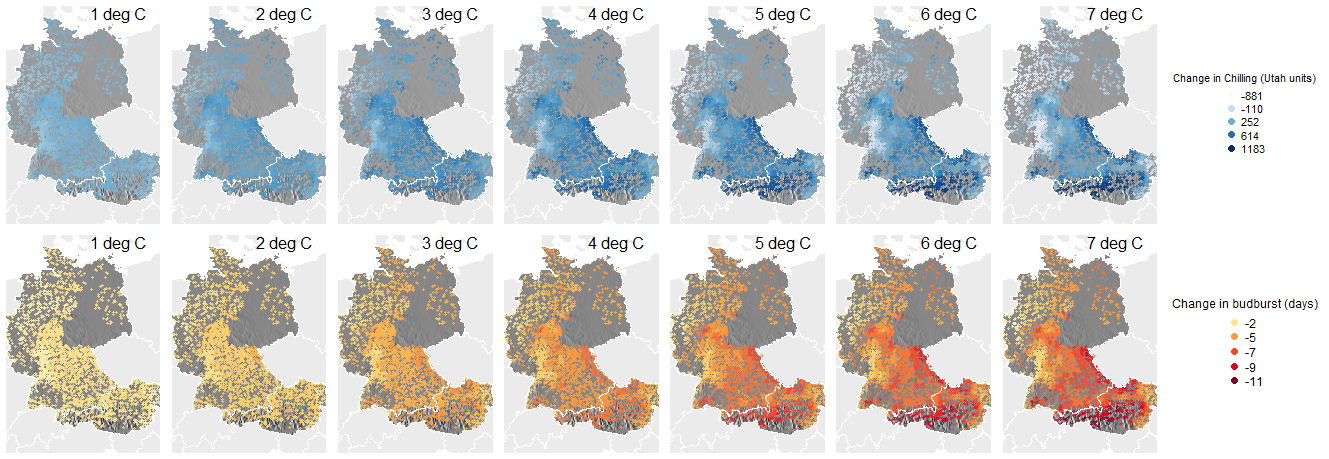
\includegraphics[width=0.75\textwidth]{..//..//analyses/bb_analysis/figures/forecasting/Heatmap_betpen_forecast_chillbb_nacho.pdf}
\caption{\textbf{Forecasted changes in chilling (top panel) and leafout for \emph{Betula pendula}(bottom panel)}, in locations included in the PEP database, where phenology dates are known for the pre-warming time period (1951-1960). Changes in chilling and budburst are calculated relative to the mean chilling and budburst dates during this pre-warming timeperiod for each location.} 
\label{fig:foremap}
\end{figure}

\newpage
\begin{figure}[h!]
\centering
\noindent 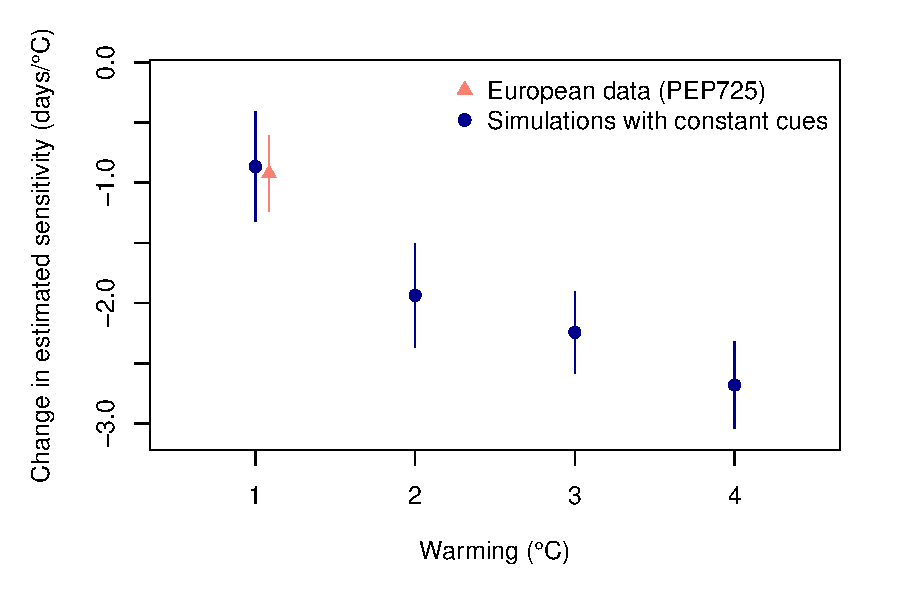
\includegraphics[width=0.75\textwidth]{..//..//analyses/bb_analysis/PEP_climate/figures/peprealandsims.pdf}
\caption{Declining sensitivities observed in long-term European data for a suite of common trees may be explained by a statistical artifact. We compared the sensitivity estimated from linear regressions of day of leafout versus mean spring temperature (estimated thus as days/$^{\circ}$C) from PEP 725 data for \emph{Betula pendula} from 45 sites (`European data') with estimated declines in simulations where the cues were held constant but spring temperatures warmed by 1-4$^{\circ}$C (`Simulations') and found the estimated temperature sensitivity measured as days/$^{\circ}$C declined even though the underlying cues had not changed, see \emph{Understanding declines in temperature sensitivity in European long-term data} in Supplement for further details.}
\label{fig:pepsims}
\end{figure}

\newpage
\begin{figure}[h!]
\centering
\noindent 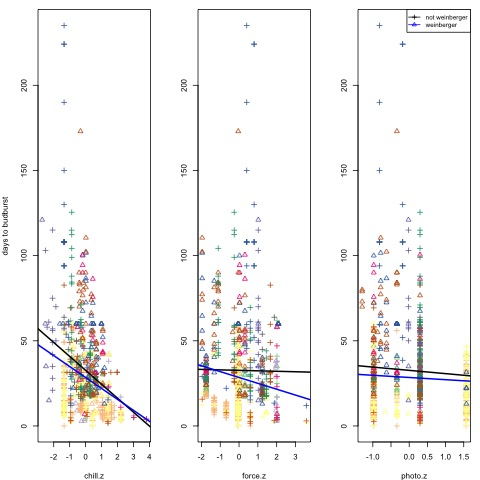
\includegraphics[width=0.75\textwidth]{..//..//analyses/figures/weinberger4supp.jpeg}
\caption{Comparision of estimated effects for environmental paremeters in for species included in both studies using the Weinberger method to simulate winter chilling and studies that did not. The effect of chilling is estimated to be weaker, and the effect of forcing stronger in Weinberger studies.}
\label{fig:weinberger}
\end{figure}

\newpage
\begin{figure}[h!]
\centering
\noindent 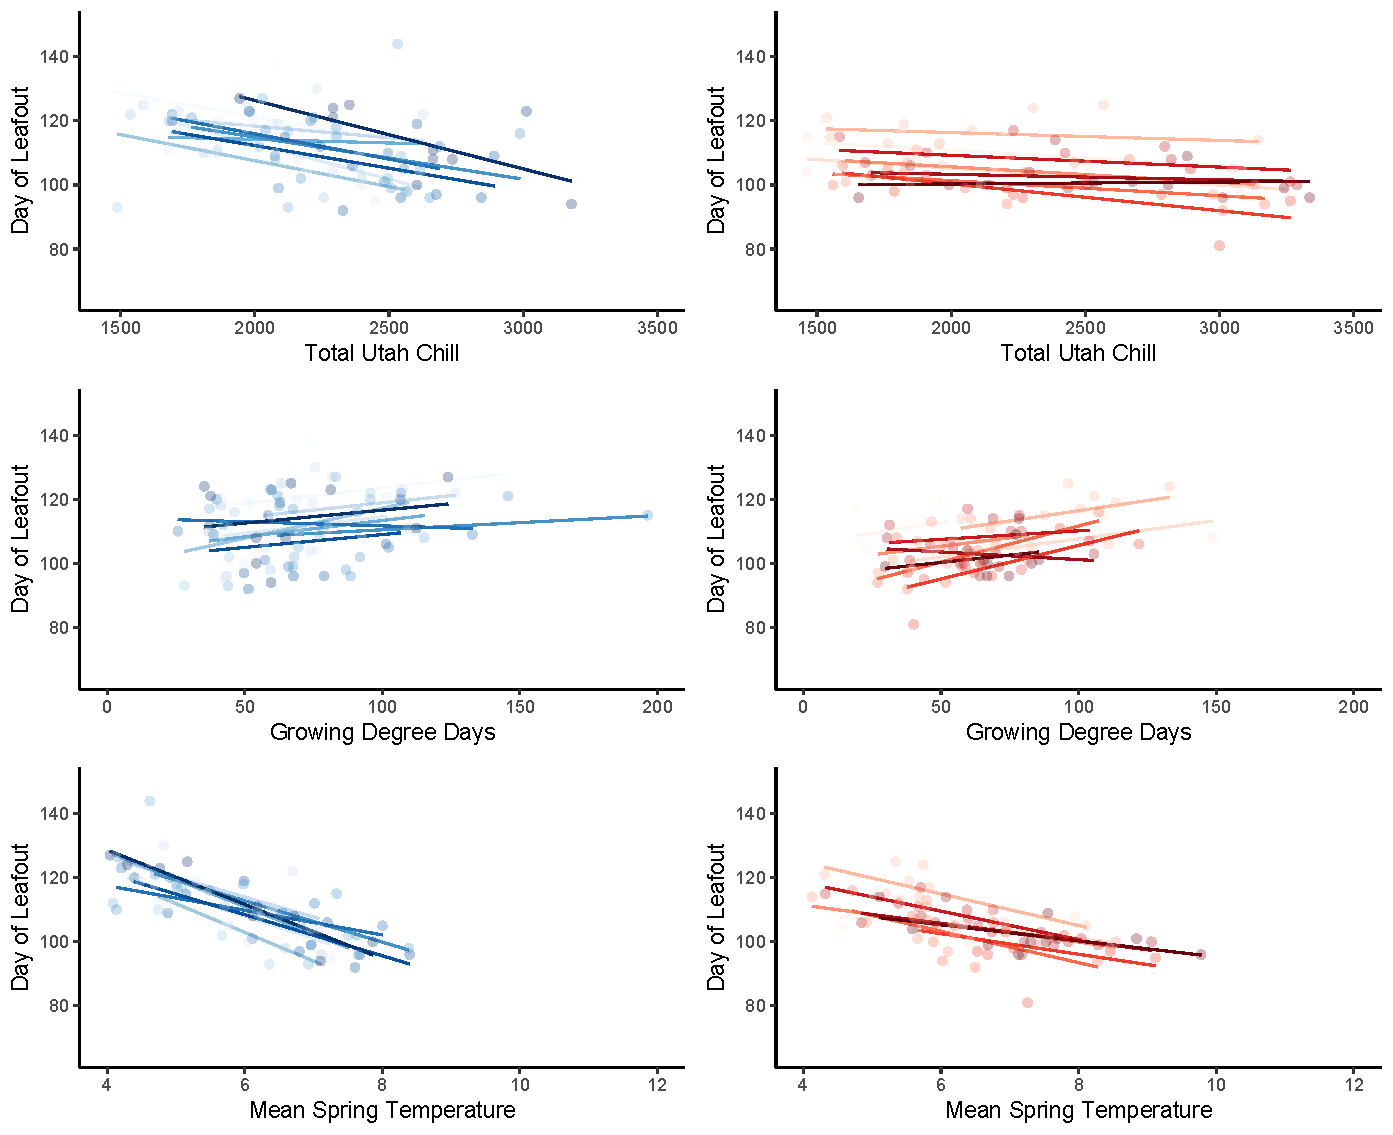
\includegraphics[width=0.75\textwidth]{..//..//analyses/bb_analysis/PEP_climate/figures/betpen_multruns_utahgddmat.pdf}
\caption{\textbf{Day of leaf out versus chilling, growing degree-days, and mean spring temperature} pre- (left panels, 1951-1961) and post- warming (right panels,2000-2010) for PEP sites in Germany where \emph{Betula pendula} phenology has been monitored for decades.}
\label{fig:pep}
\end{figure}

\newpage
\begin{figure}[h!]
\centering
\noindent 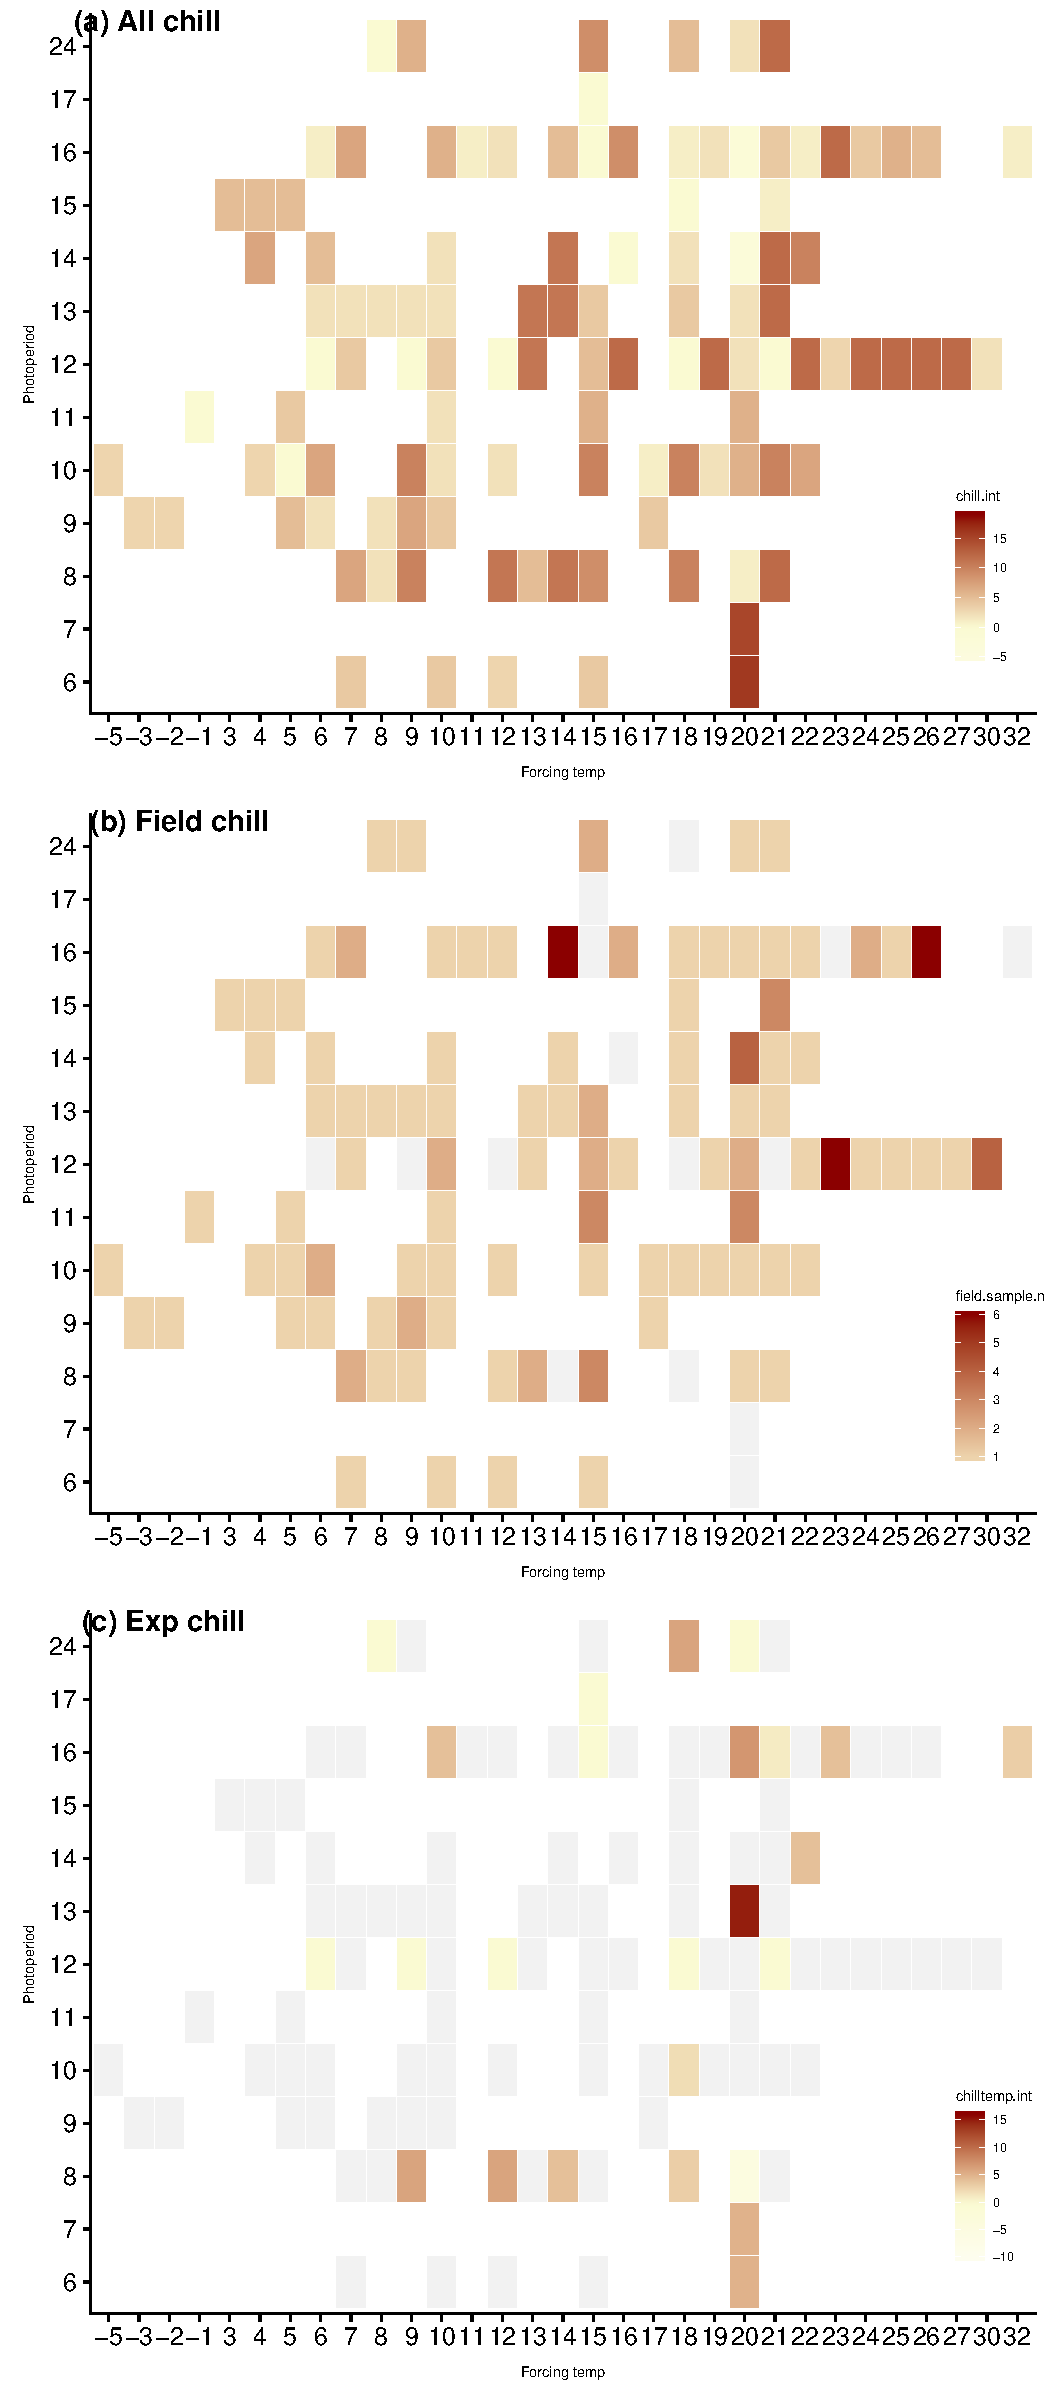
\includegraphics[width=0.75\textwidth]{..//..//analyses/bb_analysis/figures/studydesign_heat3panel.pdf}
\caption{\textbf{Heatmaps of treatments} ... need to make sure this matches the data we have ended up using!}
\label{fig:treatheatmaps} % see bb_analysis/studydesignplotsbb.R 
\end{figure}



\newpage
\begin{figure}[h!]
\centering
\noindent 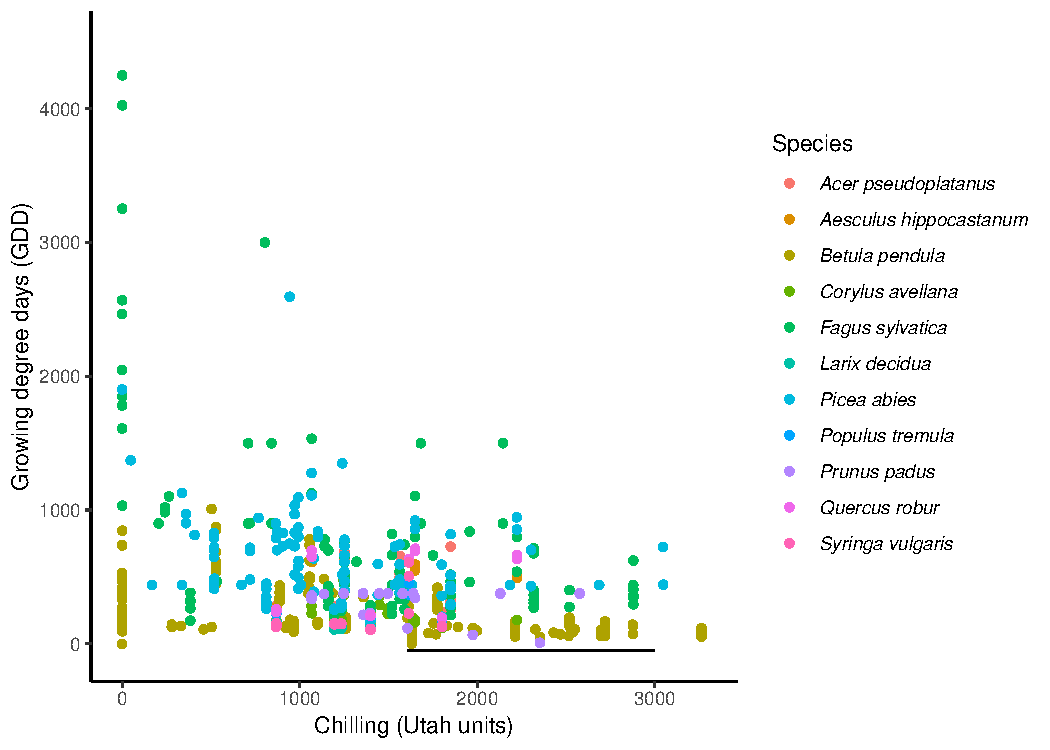
\includegraphics[width=0.75\textwidth]{..//..//analyses/bb_analysis/figures/gddbyutah_pepspp.pdf}
\caption{GDD (growing degree days) versus chill units at the time of budburst from the OSPREE database for common species in the PEP 725 long-term phenological database. The black line shows the range of chilling (10-90\% quantiles) accumulated from 1 September to 1 March for 45 sites for \emph{Betula pendula} (see also \emph{Understanding declines in temperature sensitivity in European long-term data}). We calculated GDD  here as the average daily forcing temperature multiplied by days to budburst. }
\label{fig:pepgddchill}
\end{figure}


%%%%

%%%%%%%%%%%%%%%%%%%%%%%%%%%%%%%%%%%%
\end{document}
%%%%%%%%%%%%%%%%%%%%%%%%%%%%%%%%%%%%%%%%
